\subsection{Current Infrastructure}
The LA Metro Bus currently has a few options when it comes to purchasing redeeming tickets. Riders can either purchase single-ride fares on the bus or pay using pre-purchased tokens. For both these options the rider receives a paper ticket as a proof of purchase. Another option is for metro users to purchase a TAP card from many locations across Los Angeles, and be refilled from any TAP vending machine. To use these TAP cards, users simply tap their card as they enter the bus and the appropriate fare is deduced. The initial cost for the TAP card is \$1 and can store values for up to three years. 

There is currently no competitor for the TAP concept since it is produced and run by a government agency. The current options are either using a TAP card or pay as you go. Our product would save resources, time, and create a more user friendly interface and payment options.

\subsection{Current Artifacts}
\begin{table}[h]
    \begin{tabularx}{\textwidth}{lXlr}\hline
    Artifact              & Description                                              & Status & Planned Delivery Date          \\
    \hline
    Requirements          & Written list of requirements for the app                 & Requested                   & 09/07/2013                              \\
    Architecture          & Structure of the app                                     & Requested                   & 11/01/2013                              \\
    Life-cycle plan       &  Documentation of release cycle and list of new features & Requested                   & 12/01/2013                             \\
    Feasibility evidence  & Documentation of feasibility of the application and use  & Requested                   & 12/01/2013                              \\
    \hline
    \end{tabularx}
\end{table}
\newpage
\subsection{Current Business Workflow}
\begin{figure}[h]
\centering
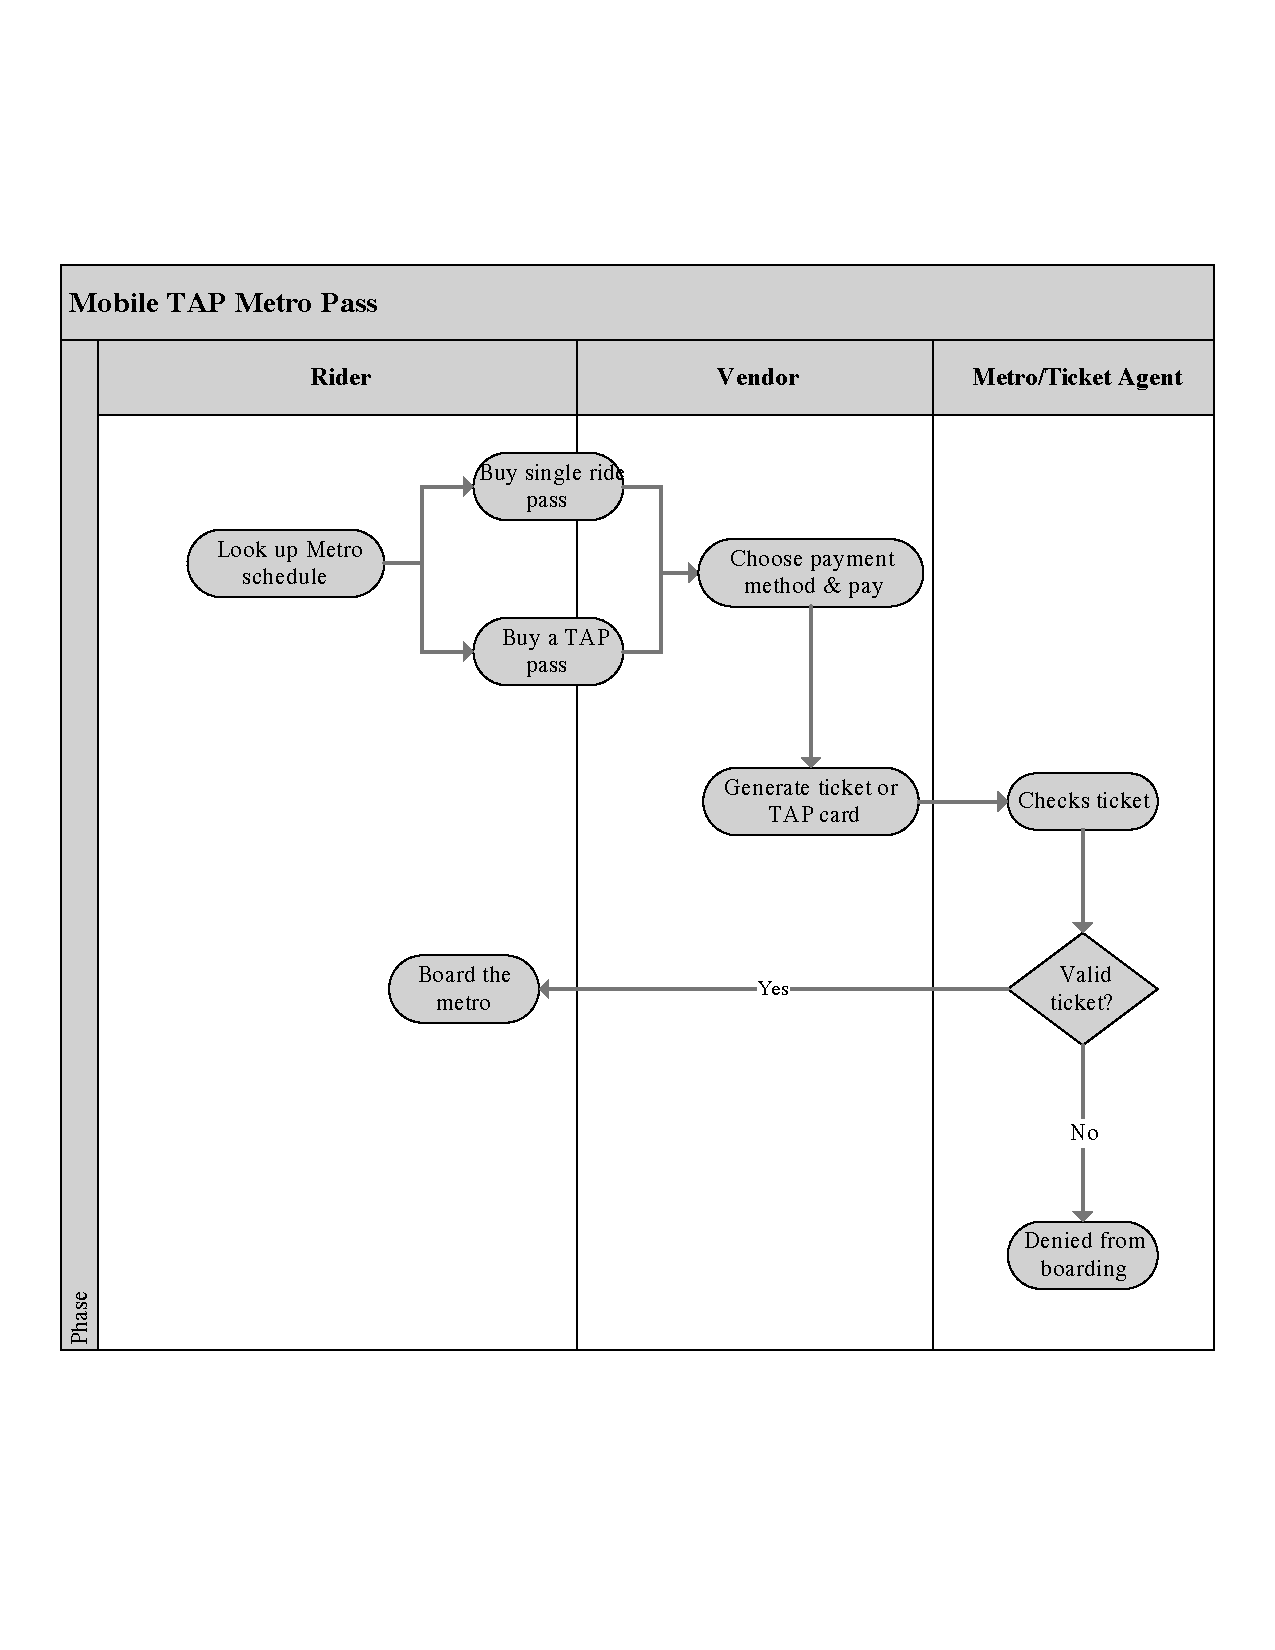
\includegraphics[scale=.5]{CIR/uml.pdf}
\end{figure}